\chapter{Introduction}

\\\\
Redaction is 'the act of removing words or information from a text before it is printed or made available to the public' (Cambride Dictionary). Information or text is often redacted when it conveys sensitive information, due to privacy and legal reasons, because the text reflects the opinion of someone, or because of the risk of commercial conflicts from the publication of data. Multiple countries have \textit{Freedom of Information Acts} \cite{USAFia}, that compel governmental bodies to release documents upon request of civilians. In The Netherlands the \textit{Wet open overheid (Woo)} \cite{WooWebsite} serves as such a law. 
\begin{figure}[h]
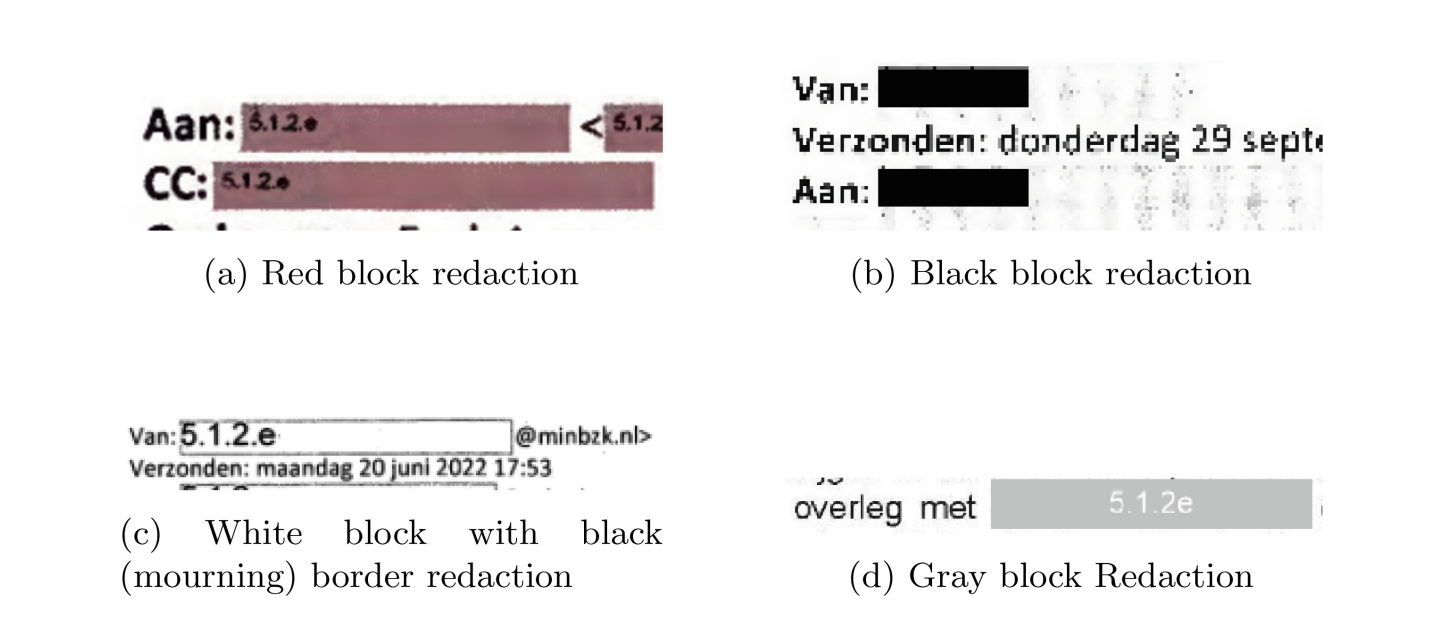
\includegraphics[width=\textwidth]{media/img.png}
\centering
\caption{Examples of four common types of text redactions which use 'black' boxes. Codes like 5.1.2.e are inserted in the redacted regions to indicate the legal ground used to redact a particular piece of text.}
\label{fig:redactionExamples}
\end{figure}\\
Two essential aspects are demanded of effective redaction. Firstly, redaction has to genuinely eliminate sensitive information from a document, leaving no residual data. Secondly, the non-redacted text has to be kept intact and visible for the reader. Striking a balance between these two aspects is challenging, as a focus on safety may compromise the readability of non-redacted text.
\begin{figure}[h]
    
    \begin{subfigure}[h]{0.5\linewidth}
        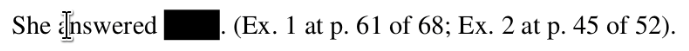
\includegraphics[width=\linewidth]{latex/media/badredaction2.png}
        \caption{A seemingly secure redaction.}
    \end{subfigure}
    \hfill
        \begin{subfigure}[h]{0.5\linewidth}
        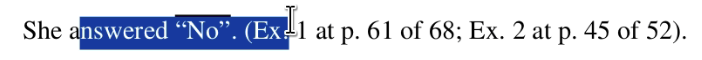
\includegraphics[width=\linewidth]{latex/media/badredaction.png}
    \caption{Selecting the box reveals the 'hidden' text.}
    \end{subfigure}%
    
\caption{An example of a bad redaction. The text has been 'redacted' by hiding it behind a black box. However, the actual text is not removed and hovering over it reveals the presence of the original text. Source: \cite{Xray2021}}
    \label{fig:redaction2}
\end{figure}\\
In the worst case all text is removed and only a sequence of images of the pages of the document are made available, particularly when first scanning in documents and then using optical character recognition (OCR) to detect text. While this enhances safety, accessibility is greatly damaged \cite{maartenMarx}, posing challenges for impaired individuals attempting to read the document.
\\\\
Figure \ref{fig:redactionExamples} illustrates four common types of text redactions using black boxes, with inserted codes indicating the legal grounds for redaction. However, ensuring complete security while maintaining accessibility can be problematic. In some instances, seemingly secure redactions, as shown in Figure \ref{fig:redaction2}, can be easily circumvented, revealing the hidden text upon closer inspection \cite{failures2019}.
\\\\
Additionally, text redaction may be broken by using subpixel-sized horizontal shifts even after to-be-redacted text has been removed \cite{bland2022story}. In particular, subpixel-sized interdependent horizontal shifts in both the redacted and non-redacted characters, can be recovered and used to effectively deredact text. Furthermore, hidden information may remain in the document after redaction, compromising text confidentiality. Embedded files, table of contents and the metadata are potential places where information may be left.
\\\\
The art is to find a middle ground which is as fast to use, easy to implement and cheap to create, and where sufficient confidentiality of information can be ensured while preserving the accessibility of the document as much as possible. 

\subsubsection{Contribution}
This project aims to establish a redaction method that strikes a balance between confidentiality and accessibility. Specifically, it presents a PDF redaction method for documents created in Microsoft Word and saved as PDFs using the '\textit{save as PDF}' functionality. The method ensures sufficient confidentiality of sensitive information and does preserve non-redacted text by directly manipulating the PDF document. 
\\\\
When applicable, the method inserts placeholder text in place of the redacted content, and non-redacted text is repositioned to fill white spaces. Additionally, hidden information is either deleted or altered when possible. Finally, following the recommendations of Maxwell Bland (one of the authors of Story Beyond the Eye \cite{bland2022story}), noise is introduced to positional information of glyphs, making it computationally more challenging to determine the redacted text. Figure \ref{fig:redactionExample} illustrates the final result of a redaction done 'correctly' with our method.
\\\\
This contribution is validated using both custom-made documents of varying complexity and real-world examples publicly released by governmental bodies in the Netherlands.

\begin{figure}[h]
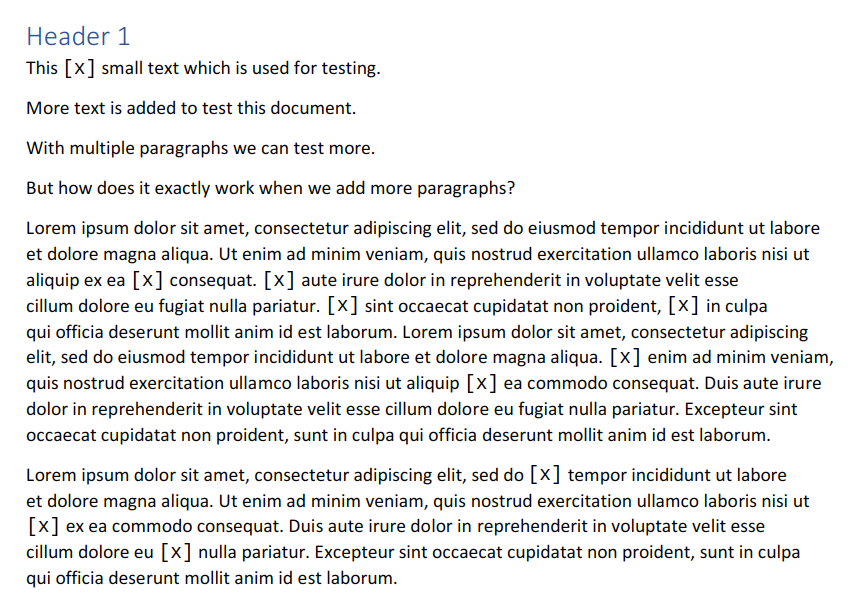
\includegraphics[width=0.9\textwidth]{latex/media/before.png}
\centering
\caption{Example of a PDF document where text has been redacted using the \textbf{Open Text Redaction Tool (OpenTRT)}. Each redacted value has been replaced with [ x ] and by manipulating the position and/or positional adjustments of text elements, possible created white spaces have been removed.}
\label{fig:redactionExample}
\end{figure}


